\chapter{Proposed approach}

\pagestyle{fancy}

\label{proposedApproach}

The main focus of this chapter is presenting detailed steps on how the solution was designed and developed. Suitably named \textbf{\textit{terra}}, the application is intended to be a great starting point for anyone that wants to create a video game using procedural generation, or for people who just want to better visualize and understand how noise and other algorithms work together to produce great results. Another use of the software could be in the educational field, where one can better understand some real-life phenomena by having an interactive "sandbox" at their disposal.\\

A vital decision that had to be made was the choice of the development environment. Programming a 3D computer graphics software from the ground up is no easy task, so these ideas were quickly dismissed. \textit{Unreal Engine 4} was a great candidate, but the amount of features that the program offers can be overwhelming, and can distract you from your goals. \textit{Unity Engine} was the perfect choice due to the fact that it is beginner friendly and there are a plethora of tutorials and guides ready to lend you a hand. One of the downsides is that \textit{Unity} products tend to be hard to optimize, due to the way things are implemented and work "behind the scenes". Because of this, one of the main focuses was improving the performance of the application and achieving a stable structure. \textit{Unity} also offers the possibility of creating a pleasant \textit{user interface}, mainly through the large amount of community assets that greatly speeds up the development process. Last but not least, the scripting language was a huge factor that contributed to the decision: programming in \textit{Unreal Engine 4} is done in \textbf{C++}, whereas \textit{Unity Engine} is based on \textbf{C\#}. While C++ is a very reliable and powerful language, I found C\# to offer some more modern features, and having its own \textit{garbage collector}, automatically managing its memory, is a huge plus.

\section{Noise generation and modeling}

The core of the entire application is the noise generating function. Unity conveniently offers a \textit{Perlin noise} implementation, that takes two parameters, the x-y axis coordinates of the sample point. Just using the output of this function alone would not suffice our needs. As we previously talked in the \textit{Theoretical aspects} chapter, there are some ways to exponentially improve the output. Creating a parametrized wrap method over the existing function was a step in the right direction, allowing us to do things such as controlling the "zoom" level, which is actually the scale of the noise map. Layering octaves to increase the detailing in the noise was done by iterating through the whole map multiple times (for each octave), multiplying the sample points with the frequency, and the {Perlin noise} result with the amplitude. Each iteration, the \textit{frequency} would increase by getting multiplied with the \textit{lacunarity} variable, while the amplitude would decrease by getting multiplied with the \textit{persistence} variable (presuming the \textit{persistence} is a value between \((0, 1)\)). A reliable method of "moving" the noise was also needed, so the sample points had to be affected by an \textit{offset}, computed as the sum of a value given as a parameter and a random value, approximated by trial and error with the random number generator offered in C\#.\\

The \textbf{[CustomEditor]} annotation tells \textit{Unity} that a class is actually an \textit{editor class}. This means that overriding the \textit{OnInspectorGUI} method, one can add custom UI elements to the editor panels, improving the workflow. The \textbf{E\_Generator} class contains the method override that specifies that a new button must be added to a \textbf{Generator} object, which is actually an empty \textit{Unity game object}, with the \textbf{Generator script} attached to it. The \textbf{Generator script} acts as a controller, handling the received data and rendering it on the screen, and the custom \textbf{"Generate"} button allows us to preview the scene after changing some settings. All the custom UI work is done exclusively to improve some quality of life aspects of the \textit{editor}, with no impact on the final product.\\

\begin{figure}[htp]
    \centering
    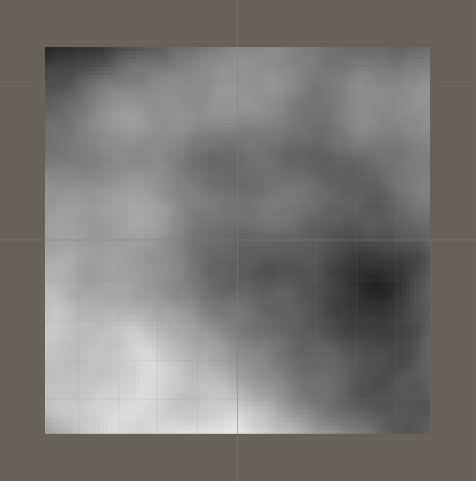
\includegraphics[width = 8cm]{figures/terraPlane.png}
    \caption{A 2D plane with a grayscale texture obtained from \([0, 1]\) noise values, generated by the \textbf{ComputeNoiseMap} method.}
    \label{fig:terraPlane}
\end{figure}

The obtained noise map was applied as a texture of grayscale colors on a plane, as seen in Figure \ref{fig:terraPlane}. This allowed us to better visualize the results and tinker with the values, until a satisfying result is obtained. The same noise map was then used to create a mesh. For every vertex of the triangles that make up the mesh, a \textbf{Vector3} data structure was used, to hold the x-y-z coordinates, where the y coordinate is actually the one that decide how much a vertex is \textit{extruded} upwards or downwards, deciding the final shape of the mesh (see Figure \ref{fig:terraMesh}). Using an \textbf{Animation curve} in a quite unorthodox way, we can control how much of an influence a certain range of values has on the final result (e.g., we could ignore all the lower noise values, thus removing all the holes that form where water should be, obtaining a flat water surface; such a decision is made only from a design perspective).

\begin{figure}[htp]
    \centering
    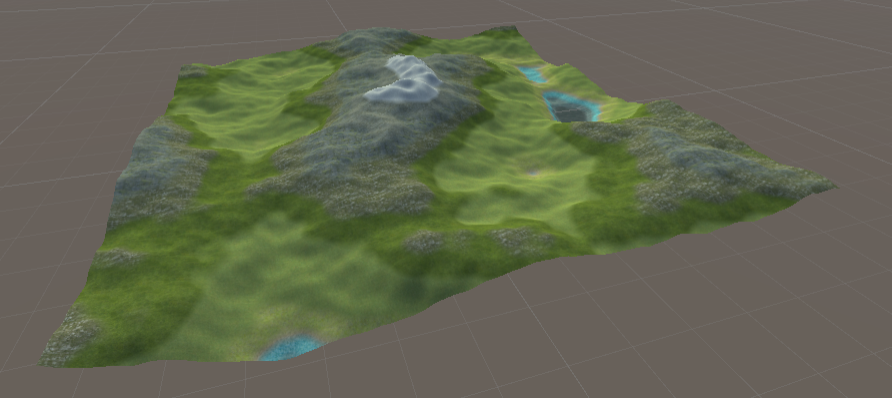
\includegraphics[width = 16cm]{figures/terraMesh.png}
    \caption{A 3D mesh generated by the \textbf{GenerateMesh} method, using a custom shader.}
    \label{fig:terraMesh}
\end{figure}

Another implemented feature is the option to use a \textbf{falloff map}, which is a configurable noise \textit{mask}, that can be applied to the main noise map, in order to isolate certain regions of interest. Using this, the application can produce landmasses surrounded entirely by water, essentially obtaining \textit{island formations}.

\section{LOD implementation}

The \textit{level of detail}, commonly known as \textbf{LOD}, has numerous types of implementations. One of the most common ones, and the one used while building the application, is reducing the polygon count (in our case, mesh triangles). Using a variable called \textbf{LOD}, the \textbf{GenerateMesh} method can loop though the mesh vertices with increments of the variable's value. A little counter-intuitive, increasing the \textbf{LOD} variable actually decreases the geometrical complexity of the mesh, but this is an easily remediable problem, being just a visual discrepancy. Anyway, the whole process results in less draw calls and better performance, Some difficulties met because of using \textit{LOD switching}, are discussed in the next subsection.

\section{Terrain chunk system}

In order to create a system that generates noise infinitely, a terrain chunk approach was chosen. The idea is to divide the whole game world into fixed size chunks, creating new ones when the player is close enough and hiding the ones that get out of range. When adding another concept such as \textit{LOD switching} on top of this, things start to get difficult. In order to maintain the game at a steady framerate, we have to use visual tricks to squeeze as much performance as we can out of the application. Lowering the number of triangles of distant chunks, progressively, is a popular method. In the \textbf{ChunkManager} script, attached to the \textbf{Generator} game object, we can associate different levels of detail to certain view distance thresholds. As seen in Figure \ref{fig:terraChunkLOD}, chunks that are farther away from the center (where the player is situated), are built from a smaller number of triangles, thing that can reduce the visual quality quite a bit. Luckily, in a real situation, the player will not be able to see the distant chunks close enough to notice the lower quality.

\begin{figure}[htp]
    \centering
    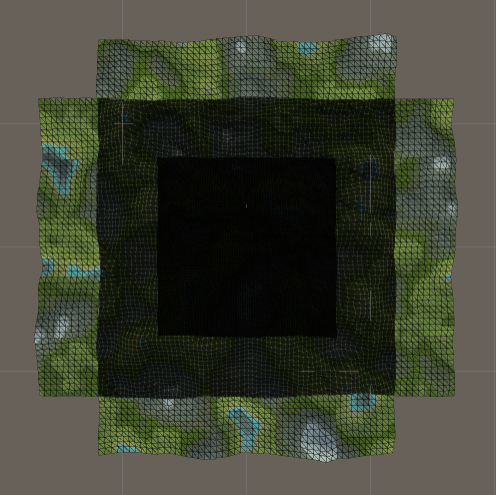
\includegraphics[width = 12cm]{figures/terraChunkLOD.png}
    \caption{A top-down, \textit{shaded wireframe} view of multiple generated terrain chunks, with different levels of detail, according to the distance from the player (center).}
    \label{fig:terraChunkLOD}
\end{figure}

One problem that is yet to be fixed is the fact that two chunks with different levels of detail will not connect perfectly. In order to remedy this, the chunk generation methods must be severely altered, and due to restricted resources, this was considered a low priority issue.

\section{Custom shader}

In early versions of the application, the terrain mesh had \textit{color-coded regions}, based on the noise value. For example, regions of the map with values between \((0.4, 0.6]\)
were colored in light green, representing flat grasslands, and the ones with values between \((0.95, 1]\) were colored in white, representing snow-covered mountain peaks. This implementation was limited due to the low triangle number of the meshes (an underlying cause is the fact that \textit{Unity Engine} supports meshes that consist of 65K vertices at most). Blocky textures, resembling \textit{Minecraft voxels} were visually unpleasant when applied to the more geometrically complex terrain. \textit{Unity} supports \textbf{HLSL}\cite{hlsl} (High Level Shading Language) and \textbf{GLSL}\cite{glsl} (OpenGL Shading Language). Programming shaders is hard, because of lot of mathematics is involved, but I managed to obtain some great results using \textbf{triplanar texturing}. This involves projecting a texture on a surface from three different directions, obtaining a mixed result, that looks good from any angle. This was a necessary measure, because when basic texture projection was used, areas such as steep slopes had stretched, deformed textures, that were very immersion-breaking.

\section{Performance optimization}

Due to the great number of computations required to render everything in real-time, at a high, constant frame rate, some performance improvements were absolutely required. The greatest optimization came from modifying the chunk generation implementation to support multithreading. Every chunk is computed and modeled on a separate thread, merging together into the final result. \textit{Deadlocks} and other \textit{concurrency problems} were not an issue, due to the fact that critical resources were protected using \textbf{locks}. Aside from critical resources, the methods involved in chunk generation could run in isolation, and produce results independently.\\

After thorough analysis, using the \textit{Unity profiler}, I discovered that some frame rate drops, commonly called \textit{spikes}, were mainly caused by the \textit{baking of collision meshes} and \textit{recalculation of normals}. \textit{Collision meshes} have to be calculated for each individual chunk, so that the player can interact physically with the surface, and not fall through it due to the gravitational pull. The only solution found was to reduce the size of the chunks, so that the \textit{baking} was done faster. Once again, this is one of \textit{Unity's} limitations, and without a custom implementation of collisions, there is not much hope of achieving better performance. The other issue was caused by the recalculation of \textit{normals}, when a new chunk was generated. \textit{Normals} are used to calculate the shading of each triangle, based on the position of the light source, and the normals of surrounding triangles. The improvement came from moving the computations for each triangle on separate threads, splitting the workload. As a side note, \textit{flatshading} is an optional mode of shading implemented, for those who like the aesthetics of it. Enabling this mode changes how the \textit{normal recalculation} works, making the triangles only take the light source into consideration.

\section{User manual}

The application's main menu offers the user three choices: "Endless Terrain", "Options" and "Quit". The first option sends the user straight into the game, where he is free to explore the infinite, procedurally generated terrain. A panel containing the hotkeys is constantly displayed on the screen, in the top-left corner. Pressing \textit{ESC} brings up a pause menu, where he can either resume the game, or quit to desktop. Back to the main menu, the user can also change some options, those being the fullscreen mode, whether he wants the terrain to be generated using the \textit{flatshading} style or not, and another option, that can toggle the \textit{falloff map}. He can also reset the settings to the defaults, if he considers so.